% Options for packages loaded elsewhere
\PassOptionsToPackage{unicode}{hyperref}
\PassOptionsToPackage{hyphens}{url}
%
\documentclass[
]{article}
\usepackage{amsmath,amssymb}
\usepackage{lmodern}
\usepackage{iftex}
\ifPDFTeX
  \usepackage[T1]{fontenc}
  \usepackage[utf8]{inputenc}
  \usepackage{textcomp} % provide euro and other symbols
\else % if luatex or xetex
  \usepackage{unicode-math}
  \defaultfontfeatures{Scale=MatchLowercase}
  \defaultfontfeatures[\rmfamily]{Ligatures=TeX,Scale=1}
\fi
% Use upquote if available, for straight quotes in verbatim environments
\IfFileExists{upquote.sty}{\usepackage{upquote}}{}
\IfFileExists{microtype.sty}{% use microtype if available
  \usepackage[]{microtype}
  \UseMicrotypeSet[protrusion]{basicmath} % disable protrusion for tt fonts
}{}
\makeatletter
\@ifundefined{KOMAClassName}{% if non-KOMA class
  \IfFileExists{parskip.sty}{%
    \usepackage{parskip}
  }{% else
    \setlength{\parindent}{0pt}
    \setlength{\parskip}{6pt plus 2pt minus 1pt}}
}{% if KOMA class
  \KOMAoptions{parskip=half}}
\makeatother
\usepackage{xcolor}
\IfFileExists{xurl.sty}{\usepackage{xurl}}{} % add URL line breaks if available
\IfFileExists{bookmark.sty}{\usepackage{bookmark}}{\usepackage{hyperref}}
\hypersetup{
  pdftitle={Report 1},
  pdfauthor={Klaudia Balcer},
  hidelinks,
  pdfcreator={LaTeX via pandoc}}
\urlstyle{same} % disable monospaced font for URLs
\usepackage[margin=1in]{geometry}
\usepackage{longtable,booktabs,array}
\usepackage{calc} % for calculating minipage widths
% Correct order of tables after \paragraph or \subparagraph
\usepackage{etoolbox}
\makeatletter
\patchcmd\longtable{\par}{\if@noskipsec\mbox{}\fi\par}{}{}
\makeatother
% Allow footnotes in longtable head/foot
\IfFileExists{footnotehyper.sty}{\usepackage{footnotehyper}}{\usepackage{footnote}}
\makesavenoteenv{longtable}
\usepackage{graphicx}
\makeatletter
\def\maxwidth{\ifdim\Gin@nat@width>\linewidth\linewidth\else\Gin@nat@width\fi}
\def\maxheight{\ifdim\Gin@nat@height>\textheight\textheight\else\Gin@nat@height\fi}
\makeatother
% Scale images if necessary, so that they will not overflow the page
% margins by default, and it is still possible to overwrite the defaults
% using explicit options in \includegraphics[width, height, ...]{}
\setkeys{Gin}{width=\maxwidth,height=\maxheight,keepaspectratio}
% Set default figure placement to htbp
\makeatletter
\def\fps@figure{htbp}
\makeatother
\setlength{\emergencystretch}{3em} % prevent overfull lines
\providecommand{\tightlist}{%
  \setlength{\itemsep}{0pt}\setlength{\parskip}{0pt}}
\setcounter{secnumdepth}{-\maxdimen} % remove section numbering
\usepackage{bbm}
\usepackage{caption}
\usepackage{tabularx}
\usepackage{booktabs}
\usepackage{graphicx}
\usepackage{amsmath}
\ifLuaTeX
  \usepackage{selnolig}  % disable illegal ligatures
\fi

\title{Report 1}
\usepackage{etoolbox}
\makeatletter
\providecommand{\subtitle}[1]{% add subtitle to \maketitle
  \apptocmd{\@title}{\par {\large #1 \par}}{}{}
}
\makeatother
\subtitle{LASSO, Ridge and ElasticNet Regression}
\author{Klaudia Balcer}
\date{12/17/2021}

\begin{document}
\maketitle

{
\setcounter{tocdepth}{2}
\tableofcontents
}
\newpage

\hypertarget{task-1}{%
\section{Task 1}\label{task-1}}

In the first task, we will compare the properties of Ordinary Least
Squares (OLS) and Ridge regression. We will consider the variance, the
bias, and the mean squared error (MSE) of \(\hat \beta\) in the
orthogonal design.

\hypertarget{theoretical-calculations-for-ridge-regression}{%
\subsection{Theoretical calculations for Ridge
Regression}\label{theoretical-calculations-for-ridge-regression}}

\begin{enumerate}
\def\labelenumi{\arabic{enumi}.}
\tightlist
\item
  \textbf{Coefficients}
\end{enumerate}

\[\hat \beta ^{RIDGE} = \frac {1}{1 + \gamma} \hat \beta ^{LS}\]

\begin{enumerate}
\def\labelenumi{\arabic{enumi}.}
\setcounter{enumi}{1}
\tightlist
\item
  \textbf{Optimal \(\gamma\) (in terms of MSE)}
\end{enumerate}

\[\gamma_{opt} = \frac {p\sigma^2} {\Vert\beta\Vert^2}\]

\begin{enumerate}
\def\labelenumi{\arabic{enumi}.}
\setcounter{enumi}{2}
\tightlist
\item
  \textbf{MSE}
\end{enumerate}

\begin{itemize}
\tightlist
\item
  general:
\end{itemize}

\[MSE(\gamma) = \frac {\gamma^2\Vert\beta\Vert^2 + p\sigma^2} {(1 + \gamma)^2}\]

\begin{itemize}
\tightlist
\item
  for optimal \(\gamma\):
\end{itemize}

\[MSE_{opt} = \frac {\Vert\beta\Vert^2 p\sigma^2} {\Vert\beta\Vert^2 + p\sigma^2} \]

\begin{enumerate}
\def\labelenumi{\arabic{enumi}.}
\setcounter{enumi}{3}
\tightlist
\item
  \textbf{Bias}
\end{enumerate}

\begin{itemize}
\tightlist
\item
  general:
\end{itemize}

\[\mathbb E [\hat \beta ^{RIDGE} - \beta] = \mathbb E \hat \beta ^{RIDGE} - \beta = \mathbb E [\frac {1}{1 + \gamma} \hat \beta ^{LS}] - \beta = \frac {1}{1 + \gamma} \mathbb E\hat \beta ^{LS} - \beta = \frac {1}{1 + \gamma}  \beta  - \beta = -\frac {\gamma}{1 + \gamma}  \beta \]

\begin{itemize}
\tightlist
\item
  for optimal \(\gamma\):
\end{itemize}

\[Bias_{opt} = -\frac {p\sigma^2}{p\sigma^2 + \Vert \beta \Vert^2} \beta \]

\begin{enumerate}
\def\labelenumi{\arabic{enumi}.}
\setcounter{enumi}{4}
\tightlist
\item
  \textbf{Variance}
\end{enumerate}

\begin{itemize}
\tightlist
\item
  general:
\end{itemize}

\[Var(\hat \beta_i^{RIDGE}) = 
  Var\Big(\frac {1}{1 +  \gamma} (\beta_i + Z_i)  \Big) = 
  \Big( \frac {1}{1 +  \gamma} \Big)^2 Var(\beta_i +  Z_i) =
  \Big( \frac {1}{1 +  \gamma} \Big)^2 Var(Z_i) = 
  \Big( \frac {1}{1 +  \gamma} \Big)^2 \sigma^2 = 
  \frac {\sigma ^2} {( 1 + \gamma) ^2}\]

\begin{itemize}
\tightlist
\item
  for optimal \(\gamma\):
\end{itemize}

\[\frac {\sigma^2 \Vert\beta\Vert^4} {(p\sigma^2 + \Vert\beta\Vert^2)^2}\]

\hypertarget{simulations}{%
\subsection{Simulations}\label{simulations}}

We will repeat the following experiment two hundred times:

\begin{itemize}
\item
  generate an orthogonal matrix \(X\) of size \(1000 \times 950\),
  generate an error term vector from standard normal distribution;
\item
  the real coefficients are: \(\beta_1, \ldots, \beta_k = 3.5\),
  \(\beta_{k+1}, \ldots, \beta_{950} = 0\) for \(k\) equal 20, 100, 200;
\item
  select tuning parameter \(\lambda\) for Ridge Regression to minimize
  the MSE of \(\hat\beta\);
\item
  build an OLS and Ridge Regression model;
\item
  evaluate the models by calculating MSE, variance and bias.
\end{itemize}

\hypertarget{results}{%
\subsection{Results}\label{results}}

\hypertarget{results-for-k20}{%
\subsubsection{Results for k=20}\label{results-for-k20}}

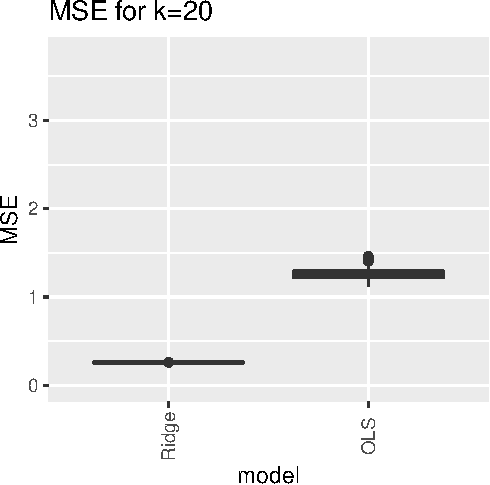
\includegraphics[width=0.8\linewidth]{report_files/figure-latex/unnamed-chunk-3-1}
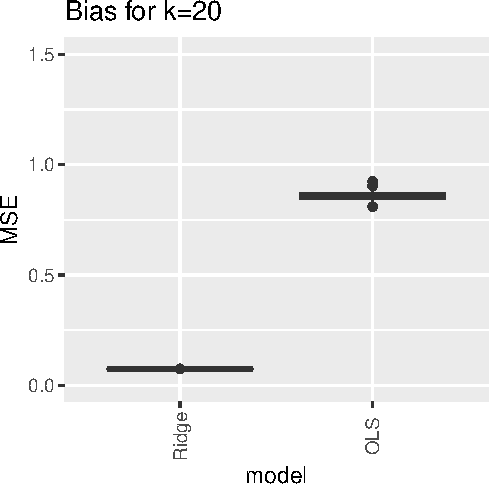
\includegraphics[width=0.8\linewidth]{report_files/figure-latex/unnamed-chunk-3-2}
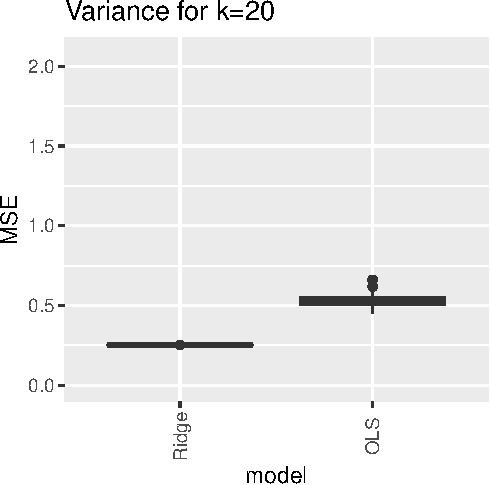
\includegraphics[width=0.8\linewidth]{report_files/figure-latex/unnamed-chunk-3-3}

\hypertarget{results-for-k100}{%
\subsubsection{Results for k=100}\label{results-for-k100}}

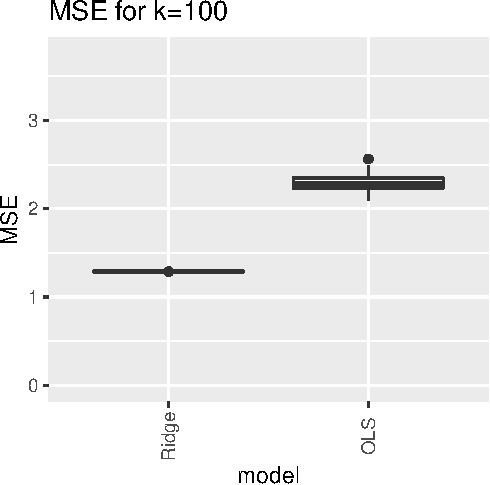
\includegraphics[width=0.8\linewidth]{report_files/figure-latex/unnamed-chunk-3-4}
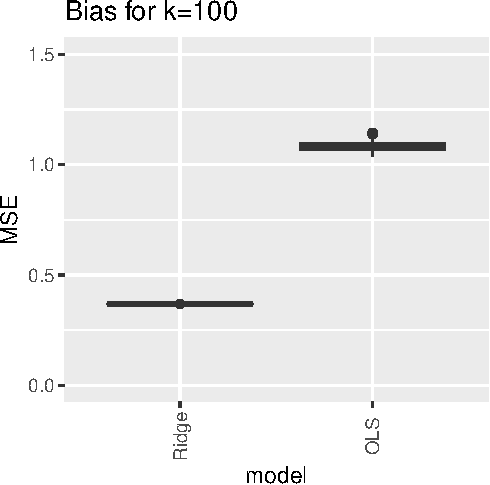
\includegraphics[width=0.8\linewidth]{report_files/figure-latex/unnamed-chunk-3-5}
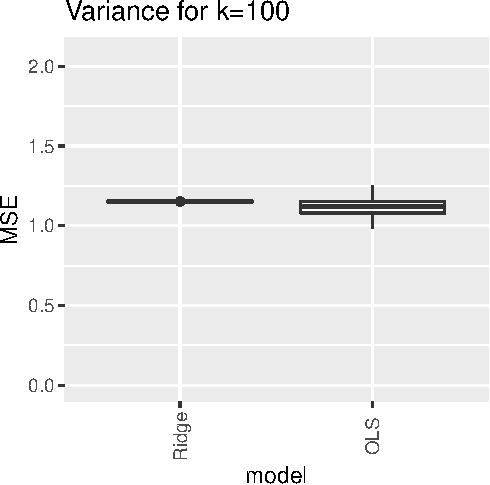
\includegraphics[width=0.8\linewidth]{report_files/figure-latex/unnamed-chunk-3-6}

\hypertarget{results-for-k200}{%
\subsubsection{Results for k=200}\label{results-for-k200}}

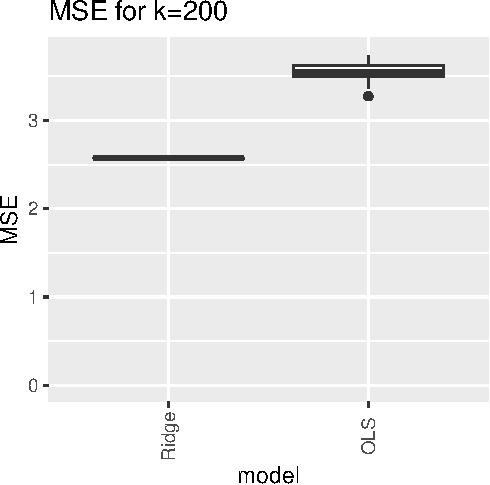
\includegraphics[width=0.8\linewidth]{report_files/figure-latex/unnamed-chunk-3-7}
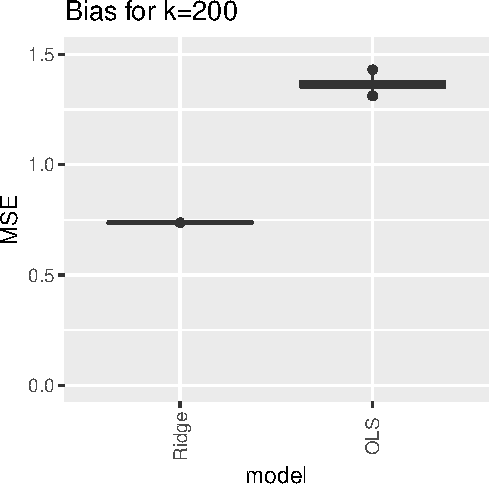
\includegraphics[width=0.8\linewidth]{report_files/figure-latex/unnamed-chunk-3-8}
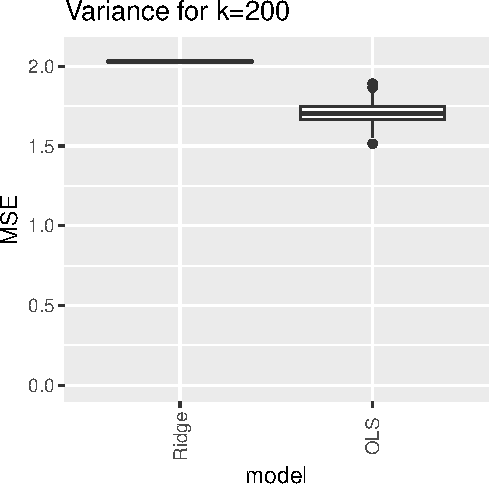
\includegraphics[width=0.8\linewidth]{report_files/figure-latex/unnamed-chunk-3-9}

\hypertarget{results-summary}{%
\subsubsection{Results summary}\label{results-summary}}

\begin{longtable}[]{@{}lrrr@{}}
\caption{Comparison of OLS and Ridge Regression}\tabularnewline
\toprule
& 20 & 100 & 200 \\
\midrule
\endfirsthead
\toprule
& 20 & 100 & 200 \\
\midrule
\endhead
MSE\_rr & 0.26 & 1.29 & 2.57 \\
bias\_rr & 0.07 & 0.37 & 0.74 \\
var\_rr & 0.25 & 1.15 & 2.03 \\
MSE\_ols & 1.26 & 2.29 & 3.58 \\
bias\_ols & 0.86 & 1.08 & 1.37 \\
var\_ols & 0.53 & 1.12 & 1.71 \\
\bottomrule
\end{longtable}

Both methods work better for small number of effects. When the signal is
sparse, Ridge outperforms OLS. When the number of significant variables
increases, the variance of Ridge also increases. For k=200, Ridge has a
greater variance than OLS. However, it has still much smaller bias (and
smaller MSE in consequence).

\hypertarget{task-2}{%
\section{Task 2}\label{task-2}}

In this and the upcoming tasks, we will compare several regression
approaches. We will compare the MSE of predictions and coefficients for
all those approaches.

\hypertarget{theoretical-calculations}{%
\subsection{Theoretical calculations}\label{theoretical-calculations}}

Prediction error for ridge regression (using SURE):

\[\widehat{PE} = RSS + 2\sigma^2\sum_{i=1}^n \frac{\lambda_i (X^TX)}{\lambda_i (X^TX) + \gamma}\]

where \(\lambda_i\) are the eigen values of
\(H=X(X^TX+\gamma I)^{-1}X^T\).

Prediction error for LASSO (using SURE):

\[\widehat{PE} = RSS + 2\sigma^2 \#\mathcal A\] where \(\#\mathcal A\)
is the number of selected variables.

\hypertarget{simulations-1}{%
\subsection{Simulations}\label{simulations-1}}

We will repeat the following experiment a hundred times:

\begin{itemize}
\item
  sample matrix \(X\) of size \(1000 \times 950\) from normal
  distribution \(\mathcal N (0, \sigma = frac 1 {\sqrt n})\), generate
  an error term vector from standard normal distribution;
\item
  the real coefficients are: \(\beta_1, \ldots, \beta_k = 3.5\),
  \(\beta_{k+1}, \ldots, \beta_{950} = 0\) for \(k\) equal 20, 100, 200;
\item
  build models:

  \begin{itemize}
  \item
    LASSO with

    \begin{itemize}
    \item
      \(\lambda\) from CV,
    \item
      \(\lambda\) from SURE;
    \end{itemize}
  \item
    Ridge Regression

    \begin{itemize}
    \item
      \(\lambda\) from CV,
    \item
      \(\lambda\) from SURE;
    \end{itemize}
  \item
    ElasticNet with \(\alpha=0.5\) and

    \begin{itemize}
    \item
      \(\lambda\) from CV,
    \item
      \(\lambda\) from SURE;
    \end{itemize}
  \item
    OLS

    \begin{itemize}
    \item
      with all variables,
    \item
      with variables selected by AIC,
    \item
      with variables selected by mBIC2.
    \end{itemize}
  \end{itemize}
\item
  evaluate the models by calculating MSE for \(\hat\beta\) and
  \(\hat Y\).
\end{itemize}

\hypertarget{results-1}{%
\subsection{Results}\label{results-1}}

\hypertarget{results-for-k20-1}{%
\subsubsection{Results for k=20}\label{results-for-k20-1}}

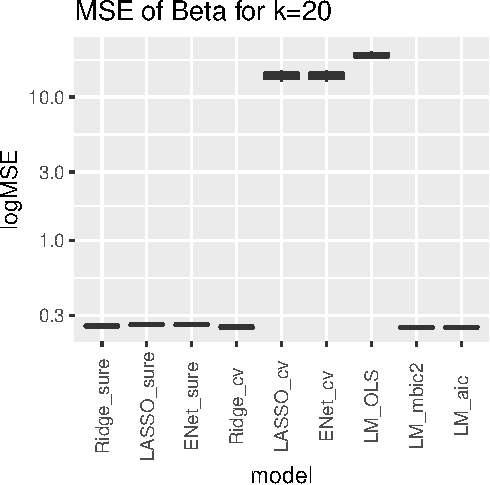
\includegraphics[width=0.8\linewidth]{report_files/figure-latex/unnamed-chunk-7-1}
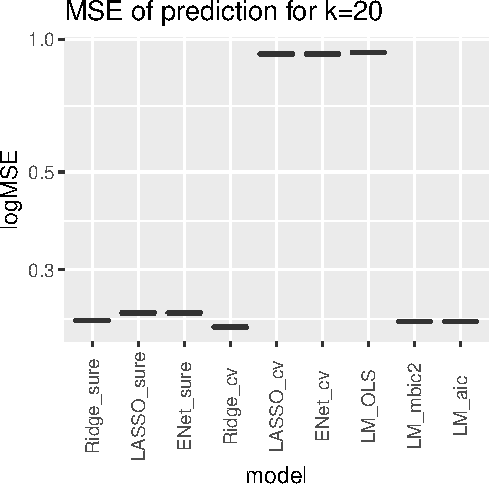
\includegraphics[width=0.8\linewidth]{report_files/figure-latex/unnamed-chunk-7-2}

\hypertarget{results-for-k100-1}{%
\subsubsection{Results for k=100}\label{results-for-k100-1}}

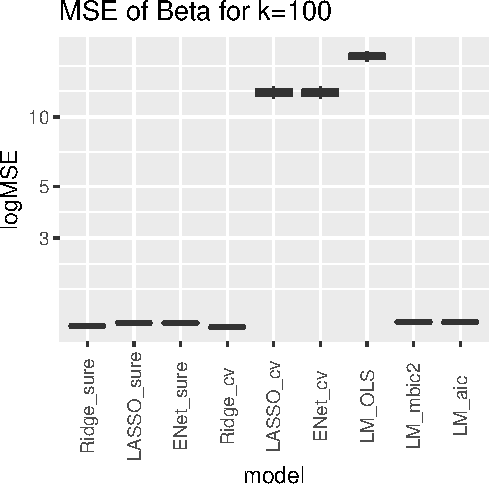
\includegraphics[width=0.8\linewidth]{report_files/figure-latex/unnamed-chunk-7-3}
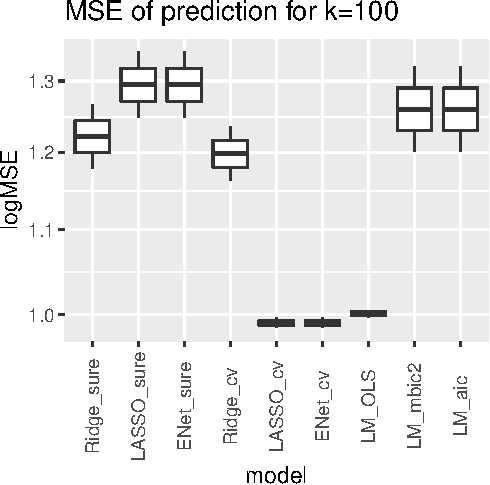
\includegraphics[width=0.8\linewidth]{report_files/figure-latex/unnamed-chunk-7-4}

\hypertarget{results-for-k200-1}{%
\subsubsection{Results for k=200}\label{results-for-k200-1}}

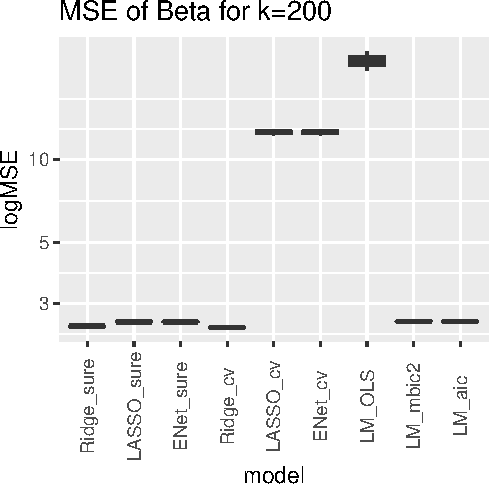
\includegraphics[width=0.8\linewidth]{report_files/figure-latex/unnamed-chunk-7-5}
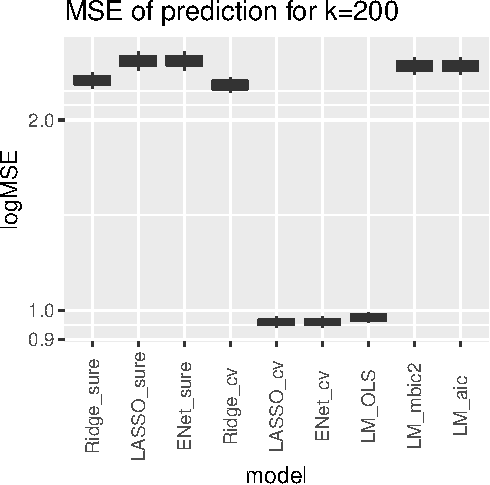
\includegraphics[width=0.8\linewidth]{report_files/figure-latex/unnamed-chunk-7-6}

\hypertarget{results-summary-1}{%
\subsubsection{Results summary}\label{results-summary-1}}

\begin{longtable}[]{@{}lrrr@{}}
\caption{MSE of Beta}\tabularnewline
\toprule
& 20 & 100 & 200 \\
\midrule
\endfirsthead
\toprule
& 20 & 100 & 200 \\
\midrule
\endhead
Ridge\_sure & 0.25 & 1.25 & 2.49 \\
LASSO\_sure & 0.26 & 1.29 & 2.58 \\
ENet\_sure & 0.26 & 1.29 & 2.58 \\
Ridge\_cv & 0.25 & 1.24 & 2.46 \\
LASSO\_cv & 14.11 & 12.75 & 12.56 \\
ENet\_cv & 14.11 & 12.75 & 12.56 \\
LM\_OLS & 19.64 & 18.28 & 22.86 \\
LM\_mbic2 & 0.25 & 1.30 & 2.59 \\
LM\_aic & 0.25 & 1.30 & 2.59 \\
\bottomrule
\end{longtable}

\begin{longtable}[]{@{}lrrr@{}}
\caption{MSE of prediction}\tabularnewline
\toprule
& 20 & 100 & 200 \\
\midrule
\endfirsthead
\toprule
& 20 & 100 & 200 \\
\midrule
\endhead
Ridge\_sure & 0.23 & 1.22 & 2.31 \\
LASSO\_sure & 0.24 & 1.30 & 2.48 \\
ENet\_sure & 0.24 & 1.30 & 2.48 \\
Ridge\_cv & 0.22 & 1.20 & 2.27 \\
LASSO\_cv & 0.93 & 0.99 & 0.96 \\
ENet\_cv & 0.93 & 0.99 & 0.96 \\
LM\_OLS & 0.93 & 1.00 & 0.97 \\
LM\_mbic2 & 0.23 & 1.26 & 2.44 \\
LM\_aic & 0.23 & 1.26 & 2.44 \\
\bottomrule
\end{longtable}

Although the 10-fold cross-validation does not estimate coefficients
precisely, its prediction properties are well and do not depend on k. In
most cases, it works at least as well as OLS. When minimizing the
Prediction Error Estimator obtained from SURE, the results are similar
to those for non-regularised linear models with preselected variables.
Results for both of these groups get worse when k increases.

\hypertarget{task-3}{%
\section{Task 3}\label{task-3}}

In this task we will repeat the previous experiment for stronger signal.

\hypertarget{simulations-2}{%
\subsection{Simulations}\label{simulations-2}}

We will repeat the following experiment a hundred times:

\begin{itemize}
\item
  sample matrix \(X\) of size \(1000 \times 950\) from normal
  distribution \(\mathcal N (0, \sigma = frac 1 {\sqrt n})\), generate
  an error term vector from standard normal distribution;
\item
  \textbf{the real coefficients are: \(\beta_1, \ldots, \beta_k = 5\),
  \(\beta_{k+1}, \ldots, \beta_{950} = 0\) for \(k\) equal 20, 100,
  200;}
\item
  build models:

  \begin{itemize}
  \item
    LASSO with

    \begin{itemize}
    \item
      \(\lambda\) from CV,
    \item
      \(\lambda\) from SURE;
    \end{itemize}
  \item
    Ridge Regression

    \begin{itemize}
    \item
      \(\lambda\) from CV,
    \item
      \(\lambda\) from SURE;
    \end{itemize}
  \item
    ElasticNet with \(\alpha=0.5\) and

    \begin{itemize}
    \item
      \(\lambda\) from CV,
    \item
      \(\lambda\) from SURE;
    \end{itemize}
  \item
    OLS

    \begin{itemize}
    \item
      with all variables,
    \item
      with variables selected by AIC,
    \item
      with variables selected by mBIC2.
    \end{itemize}
  \end{itemize}
\item
  evaluate the models by calculating MSE for \(\hat\beta\) and
  \(\hat Y\).
\end{itemize}

\hypertarget{results-2}{%
\subsection{Results}\label{results-2}}

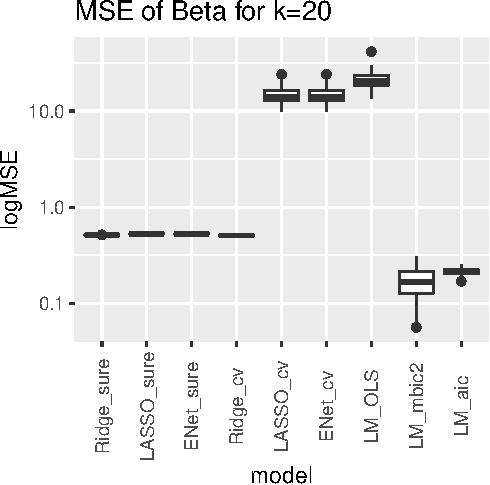
\includegraphics[width=0.8\linewidth]{report_files/figure-latex/unnamed-chunk-10-1}
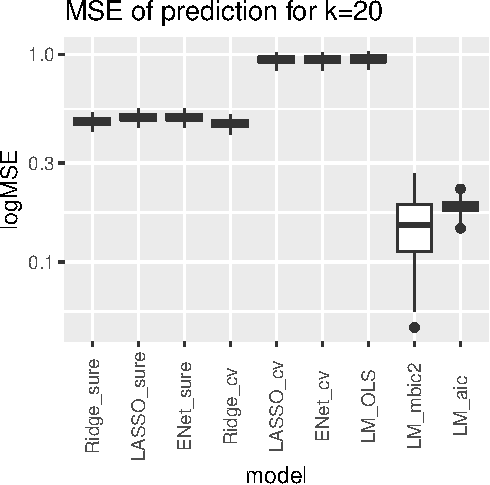
\includegraphics[width=0.8\linewidth]{report_files/figure-latex/unnamed-chunk-10-2}
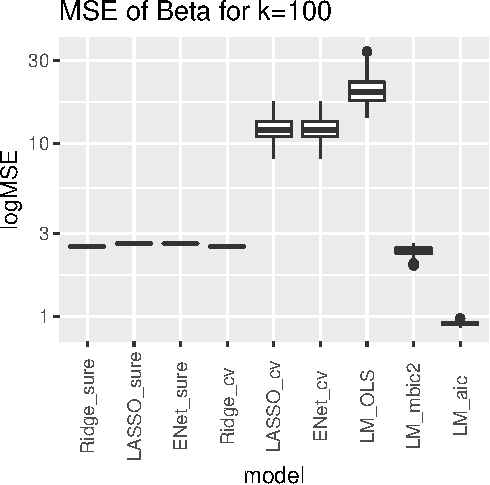
\includegraphics[width=0.8\linewidth]{report_files/figure-latex/unnamed-chunk-10-3}
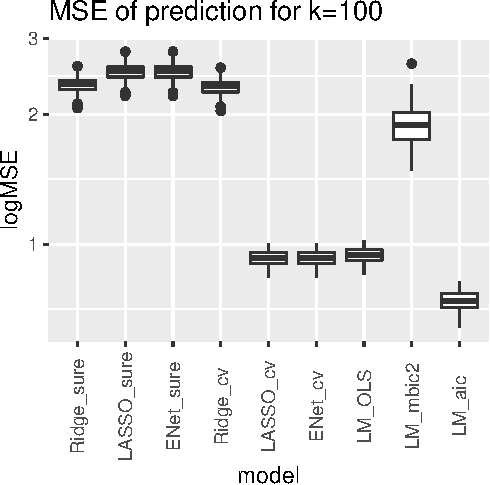
\includegraphics[width=0.8\linewidth]{report_files/figure-latex/unnamed-chunk-10-4}
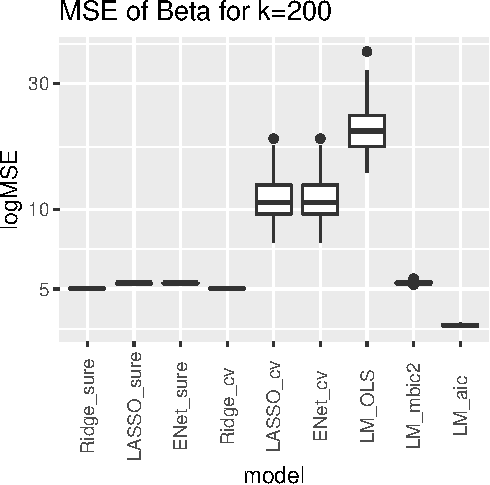
\includegraphics[width=0.8\linewidth]{report_files/figure-latex/unnamed-chunk-10-5}
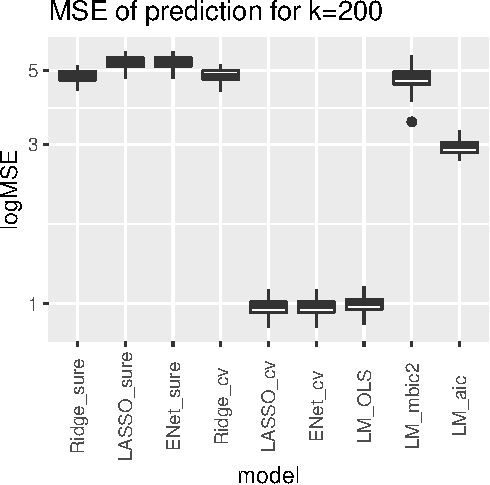
\includegraphics[width=0.8\linewidth]{report_files/figure-latex/unnamed-chunk-10-6}

\begin{longtable}[]{@{}lrrr@{}}
\caption{MSE of Beta}\tabularnewline
\toprule
& 20 & 100 & 200 \\
\midrule
\endfirsthead
\toprule
& 20 & 100 & 200 \\
\midrule
\endhead
Ridge\_sure & 0.51 & 2.54 & 5.02 \\
LASSO\_sure & 0.53 & 2.63 & 5.26 \\
ENet\_sure & 0.53 & 2.63 & 5.26 \\
Ridge\_cv & 0.51 & 2.53 & 5.03 \\
LASSO\_cv & 14.62 & 12.16 & 11.11 \\
ENet\_cv & 14.62 & 12.16 & 11.11 \\
LM\_OLS & 21.20 & 20.47 & 20.47 \\
LM\_mbic2 & 0.17 & 2.38 & 5.29 \\
LM\_aic & 0.21 & 0.91 & 3.66 \\
\bottomrule
\end{longtable}

\begin{longtable}[]{@{}lrrr@{}}
\caption{MSE of prediction}\tabularnewline
\toprule
& 20 & 100 & 200 \\
\midrule
\endfirsthead
\toprule
& 20 & 100 & 200 \\
\midrule
\endhead
Ridge\_sure & 0.48 & 2.34 & 4.82 \\
LASSO\_sure & 0.50 & 2.51 & 5.28 \\
ENet\_sure & 0.50 & 2.51 & 5.28 \\
Ridge\_cv & 0.47 & 2.32 & 4.84 \\
LASSO\_cv & 0.94 & 0.93 & 0.98 \\
ENet\_cv & 0.94 & 0.93 & 0.98 \\
LM\_OLS & 0.95 & 0.94 & 1.00 \\
LM\_mbic2 & 0.15 & 1.90 & 4.75 \\
LM\_aic & 0.19 & 0.74 & 2.96 \\
\bottomrule
\end{longtable}

OLS with preselected variables got better in sparse cases. All other
results became worse.

\hypertarget{task-4}{%
\section{Task 4}\label{task-4}}

\hypertarget{simulations-a}{%
\subsection{Simulations a}\label{simulations-a}}

We will repeat the following experiment a hundred times:

\begin{itemize}
\item
  sample matrix \(X\) of size \(1000 \times 950\) from multivariate
  normal distribution
  \(\mathcal N_n (0, \Sigma = 0.5 + 0.5*\mathbbm 1 {i=1})\), generate an
  error term vector from standard normal distribution;
\item
  the real coefficients are: \(\beta_1, \ldots, \beta_k = 3.5\),
  \(\beta_{k+1}, \ldots, \beta_{950} = 0\) for \(k\) equal 20, 100, 200;
\item
  build models:

  \begin{itemize}
  \item
    LASSO with

    \begin{itemize}
    \item
      \(\lambda\) from CV,
    \item
      \(\lambda\) from SURE;
    \end{itemize}
  \item
    Ridge Regression

    \begin{itemize}
    \item
      \(\lambda\) from CV,
    \item
      \(\lambda\) from SURE;
    \end{itemize}
  \item
    ElasticNet with \(\alpha=0.5\) and

    \begin{itemize}
    \item
      \(\lambda\) from CV,
    \item
      \(\lambda\) from SURE;
    \end{itemize}
  \item
    OLS

    \begin{itemize}
    \item
      with all variables,
    \item
      with variables selected by AIC,
    \item
      with variables selected by mBIC2.
    \end{itemize}
  \end{itemize}
\item
  evaluate the models by calculating MSE for \(\hat\beta\) and
  \(\hat Y\).
\end{itemize}

\hypertarget{simulations-b}{%
\subsection{Simulations b}\label{simulations-b}}

We will repeat the following experiment ten times:

\begin{itemize}
\item
  sample matrix \(X\) of size \(1000 \times 950\) from multivariate
  normal distribution
  \(\mathcal N_n (0, \Sigma = 0.5 + 0.5*\mathbbm 1 {i=1})\), generate an
  error term vector from standard normal distribution;
\item
  the real coefficients are: \(\beta_1, \ldots, \beta_k = 5\),
  \(\beta_{k+1}, \ldots, \beta_{950} = 0\) for \(k\) equal 20, 100, 200;
\item
  build models:

  \begin{itemize}
  \item
    LASSO with

    \begin{itemize}
    \item
      \(\lambda\) from CV,
    \item
      \(\lambda\) from SURE;
    \end{itemize}
  \item
    Ridge Regression

    \begin{itemize}
    \item
      \(\lambda\) from CV,
    \item
      \(\lambda\) from SURE;
    \end{itemize}
  \item
    ElasticNet with \(\alpha=0.5\) and

    \begin{itemize}
    \item
      \(\lambda\) from CV,
    \item
      \(\lambda\) from SURE;
    \end{itemize}
  \item
    OLS

    \begin{itemize}
    \item
      with all variables,
    \item
      with variables selected by AIC,
    \item
      with variables selected by mBIC2.
    \end{itemize}
  \end{itemize}
\item
  evaluate the models by calculating MSE for \(\hat\beta\) and
  \(\hat Y\).
\end{itemize}

In this and all next tasks, the AIC and mBIC2 criteria were used in the
fast forward procedure (which may be suboptimal).

\emph{Please note that the number of iterations is lower than expected
(100) because of the high time complexity of the task.}

\hypertarget{results-b}{%
\subsection{Results b}\label{results-b}}

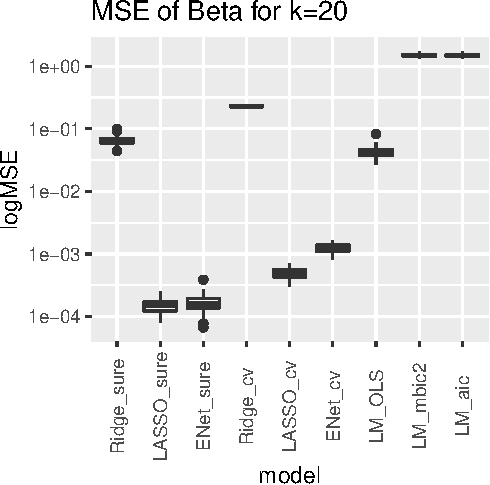
\includegraphics[width=0.8\linewidth]{report_files/figure-latex/unnamed-chunk-15-1}
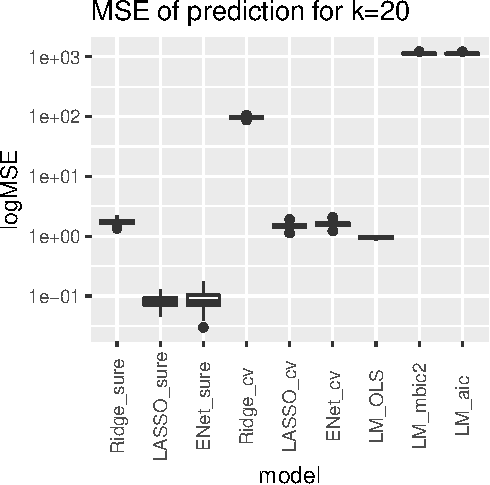
\includegraphics[width=0.8\linewidth]{report_files/figure-latex/unnamed-chunk-15-2}
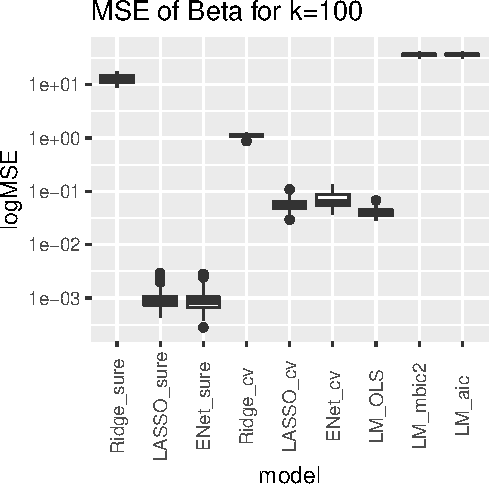
\includegraphics[width=0.8\linewidth]{report_files/figure-latex/unnamed-chunk-15-3}
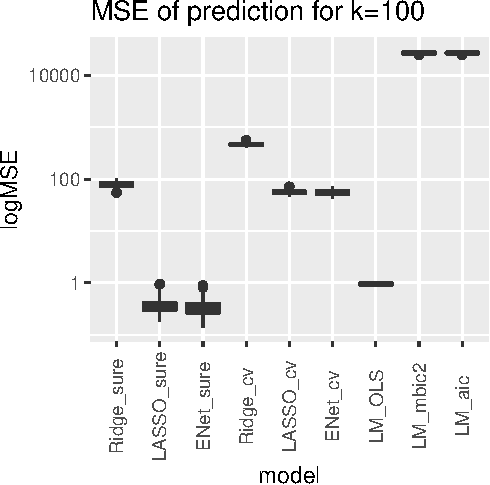
\includegraphics[width=0.8\linewidth]{report_files/figure-latex/unnamed-chunk-15-4}
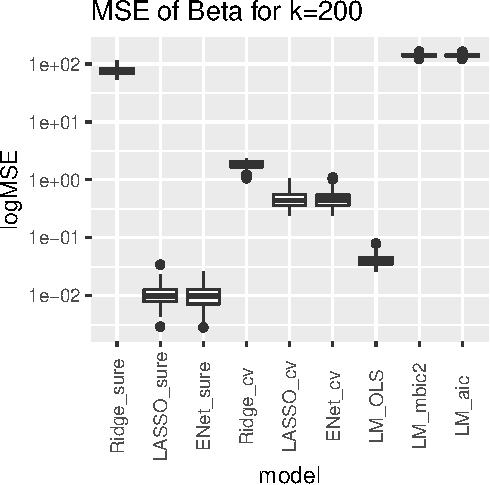
\includegraphics[width=0.8\linewidth]{report_files/figure-latex/unnamed-chunk-15-5}
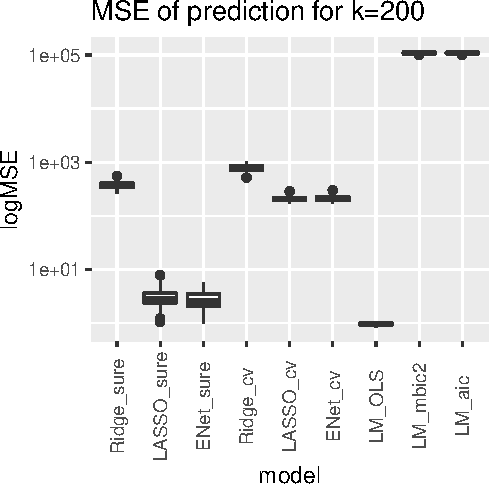
\includegraphics[width=0.8\linewidth]{report_files/figure-latex/unnamed-chunk-15-6}

\begin{longtable}[]{@{}lrrr@{}}
\caption{MSE of Beta}\tabularnewline
\toprule
& 20 & 100 & 200 \\
\midrule
\endfirsthead
\toprule
& 20 & 100 & 200 \\
\midrule
\endhead
Ridge\_sure & 0.06 & 13.11 & 76.26 \\
LASSO\_sure & 0.00 & 0.00 & 0.01 \\
ENet\_sure & 0.00 & 0.00 & 0.01 \\
Ridge\_cv & 0.23 & 1.09 & 1.83 \\
LASSO\_cv & 0.00 & 0.06 & 0.48 \\
ENet\_cv & 0.00 & 0.07 & 0.49 \\
LM\_OLS & 0.04 & 0.04 & 0.04 \\
LM\_mbic2 & 1.48 & 36.15 & 141.13 \\
LM\_aic & 1.48 & 36.15 & 141.13 \\
\bottomrule
\end{longtable}

\begin{longtable}[]{@{}lrrr@{}}
\caption{MSE of prediction}\tabularnewline
\toprule
& 20 & 100 & 200 \\
\midrule
\endfirsthead
\toprule
& 20 & 100 & 200 \\
\midrule
\endhead
Ridge\_sure & 1.76 & 79.34 & 375.45 \\
LASSO\_sure & 0.08 & 0.38 & 3.00 \\
ENet\_sure & 0.09 & 0.35 & 2.80 \\
Ridge\_cv & 96.48 & 466.78 & 784.16 \\
LASSO\_cv & 1.49 & 55.65 & 207.95 \\
ENet\_cv & 1.60 & 55.38 & 208.57 \\
LM\_OLS & 0.95 & 0.94 & 0.95 \\
LM\_mbic2 & 1125.48 & 27233.39 & 108062.81 \\
LM\_aic & 1125.48 & 27233.39 & 108062.81 \\
\bottomrule
\end{longtable}

When the variables are dependent, the task becomes much more
complicated. We got satisfying results for methods performing L1
penalization (LASSO and ENet). Good predictions from OLS. Ridge performs
poorly, OLS with preselected variables cannot handle this case.

\hypertarget{results-b-1}{%
\subsection{Results b}\label{results-b-1}}

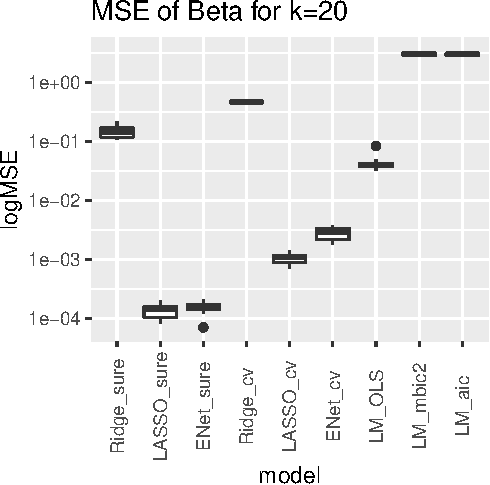
\includegraphics[width=0.8\linewidth]{report_files/figure-latex/unnamed-chunk-16-1}
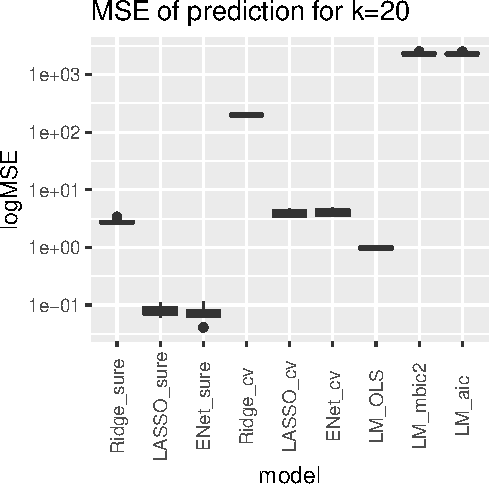
\includegraphics[width=0.8\linewidth]{report_files/figure-latex/unnamed-chunk-16-2}
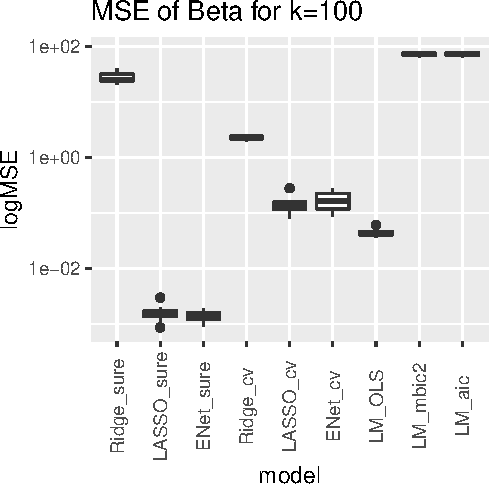
\includegraphics[width=0.8\linewidth]{report_files/figure-latex/unnamed-chunk-16-3}
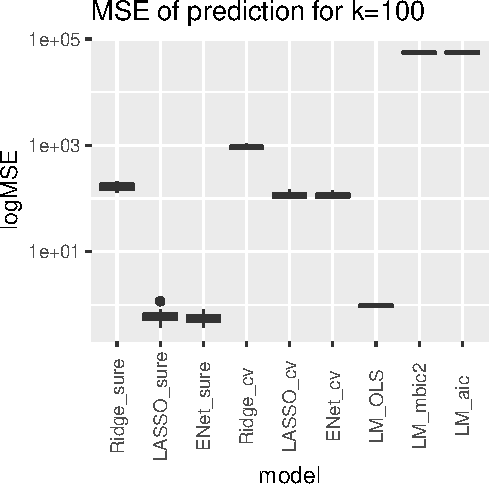
\includegraphics[width=0.8\linewidth]{report_files/figure-latex/unnamed-chunk-16-4}
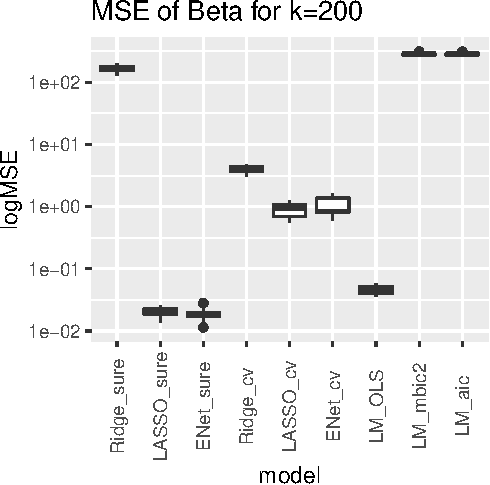
\includegraphics[width=0.8\linewidth]{report_files/figure-latex/unnamed-chunk-16-5}
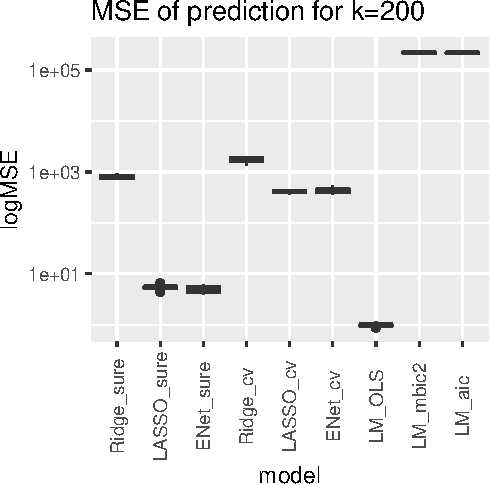
\includegraphics[width=0.8\linewidth]{report_files/figure-latex/unnamed-chunk-16-6}

\begin{longtable}[]{@{}lrrr@{}}
\caption{MSE of Beta}\tabularnewline
\toprule
& 20 & 100 & 200 \\
\midrule
\endfirsthead
\toprule
& 20 & 100 & 200 \\
\midrule
\endhead
Ridge\_sure & 0.15 & 27.67 & 168.05 \\
LASSO\_sure & 0.00 & 0.00 & 0.02 \\
ENet\_sure & 0.00 & 0.00 & 0.02 \\
Ridge\_cv & 0.47 & 2.26 & 3.98 \\
LASSO\_cv & 0.00 & 0.14 & 0.91 \\
ENet\_cv & 0.00 & 0.17 & 1.03 \\
LM\_OLS & 0.04 & 0.04 & 0.05 \\
LM\_mbic2 & 3.01 & 71.82 & 284.38 \\
LM\_aic & 3.01 & 71.82 & 284.38 \\
\bottomrule
\end{longtable}

\begin{longtable}[]{@{}lrrr@{}}
\caption{MSE of prediction}\tabularnewline
\toprule
& 20 & 100 & 200 \\
\midrule
\endfirsthead
\toprule
& 20 & 100 & 200 \\
\midrule
\endhead
Ridge\_sure & 2.78 & 167.80 & 794.44 \\
LASSO\_sure & 0.08 & 0.63 & 5.43 \\
ENet\_sure & 0.07 & 0.57 & 4.95 \\
Ridge\_cv & 198.10 & 949.09 & 1708.51 \\
LASSO\_cv & 3.91 & 116.25 & 408.13 \\
ENet\_cv & 4.02 & 115.37 & 431.43 \\
LM\_OLS & 0.97 & 0.96 & 0.97 \\
LM\_mbic2 & 2302.45 & 55565.47 & 216576.33 \\
LM\_aic & 2302.45 & 55565.47 & 216576.33 \\
\bottomrule
\end{longtable}

For stronger signals, the observations from the previous example are
further highlighted.

\hypertarget{task-5}{%
\section{Task 5}\label{task-5}}

In the fifth task we will ilustrate the irrepresentability nad
identifiability properties.

\hypertarget{theoretical-descritpion}{%
\subsection{Theoretical descritpion}\label{theoretical-descritpion}}

Irrepresentability condition:

\[\Vert X_{\bar I}^TX_I  (X_I^TX_I)^{-1}S_I \Vert_{\infty} \leq 1\]

Identifiability condition:

\[X\gamma = X\beta \text{ and } \gamma \neq \beta \text{ then } \Vert\gamma\Vert_1 > \Vert\beta\Vert_1\]

\hypertarget{simulation}{%
\subsection{Simulation}\label{simulation}}

\begin{itemize}
\item
  generate design matrix \(X\) fo size \(100 \times 200\) form the
  normal distribution \(\mathcal N (0, \sigma = 0.1)\);
\item
  find the maximal \(k^{IR}\) for which the LASSO irrepresentability
  condition holds;
\item
  find the maximal \(k^{ID}\) for which the LASSO identifiability
  condition holds;
\item
  generate the vectors of coefficients:

  \begin{itemize}
  \tightlist
  \item
    \(\beta_1, \ldots, \beta_k^{IR} = 20\),
    \(\beta_{k+1}, \ldots, \beta_{200} = 0\),
  \item
    \(\beta_1, \ldots, \beta_k^{ID} = 20\),
    \(\beta_{k+1}, \ldots, \beta_{200} = 0\),
  \item
    \(\beta_1, \ldots, \beta_k^{ID} = 20\),
    \(\beta_{k+1}, \ldots, \beta_{200} = 0\);
  \end{itemize}
\item
  generate an error term from the standard normal distribution; for each
  of the above vectors, calculate the values of dependent variable
  \(Y\);
\item
  provide scatter plots for betas and their estimators.
\end{itemize}

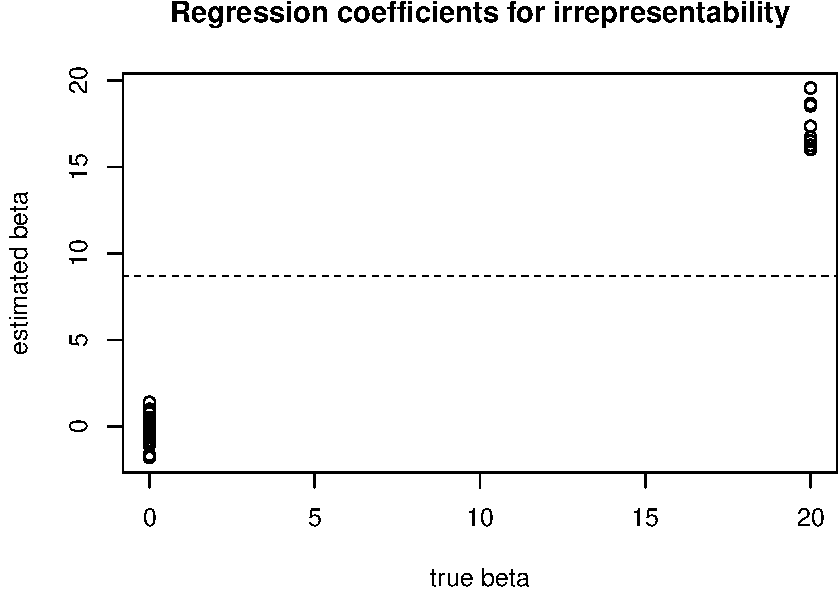
\includegraphics[width=0.8\linewidth]{report_files/figure-latex/unnamed-chunk-17-1}

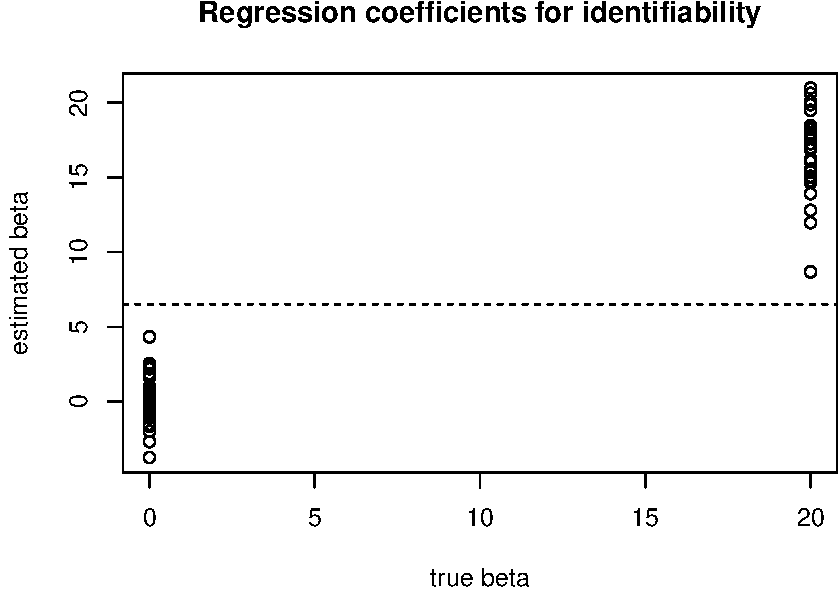
\includegraphics[width=0.8\linewidth]{report_files/figure-latex/unnamed-chunk-17-2}

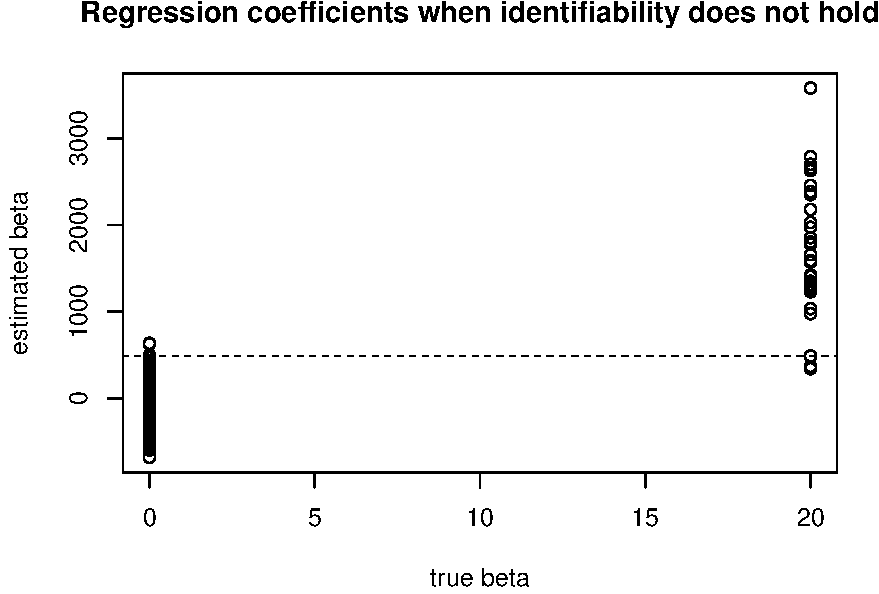
\includegraphics[width=0.8\linewidth]{report_files/figure-latex/unnamed-chunk-17-3}

As we can see in the above scatter plots, we can separate zero and
nonzero elements of the beta vector when the irrepresentability and
identifiability conditions hold. However, we cannot separate when the
identifiability condition does not hold.

\hypertarget{task-6}{%
\section{Task 6}\label{task-6}}

In this task, we will apply techniques considered before to a real world
example. We will predict the expression level of gene one using the
expression levels of 3220 other genes.

\hypertarget{implementation}{%
\subsection{Implementation}\label{implementation}}

First we split the data into train (180 individuals) and test (30
individuals) set. Then we will build LASSO, RIdge and ENet models using
lambda from cross-validation. First, we will build models using all
variables, then we will build models using only preselected variables.

\hypertarget{results-3}{%
\subsection{Results}\label{results-3}}

\begin{longtable}[]{@{}lrrr@{}}
\caption{Evaluation of models build on all variables.}\tabularnewline
\toprule
& Vars & RMSE & MAPE \\
\midrule
\endfirsthead
\toprule
& Vars & RMSE & MAPE \\
\midrule
\endhead
Ridge & 2304 & 0.2 & 1.13 \\
LASSO & 55 & 0.2 & 1.18 \\
ENet & 74 & 0.2 & 1.21 \\
\bottomrule
\end{longtable}

\begin{longtable}[]{@{}lrrr@{}}
\caption{Evaluation of models build on preselected
variables.}\tabularnewline
\toprule
& Vars & RMSE & MAPE \\
\midrule
\endfirsthead
\toprule
& Vars & RMSE & MAPE \\
\midrule
\endhead
Ridge & 295 & 0.2 & 1.12 \\
LASSO & 27 & 0.2 & 1.12 \\
ENet & 35 & 0.2 & 1.11 \\
\bottomrule
\end{longtable}

On both bases, Ridge Regression uses almost all available variables. It
has similar results with and without preselecting variables. LASSO and
ElasticNet perform better after preselecting variables; LASSO selects
the lowest number od variables, ENet has the lowest Mean Absolute
Percentage Error (MAPE).

\end{document}
